\lecture{5}{8. September 2025}{Differential Analysis I: Mass conservation}

\exercise{5.1}
Determine which of the following velocity distributions are possibly three-dimensional incompressible flows.

\paragraph{(a)}
\[ 
u = 2 y^2 + 2xz: \quad v = -2xy + 6x^2 yz; \quad w = 3x^2z^2 + x^3y^{4}
.\]
\bigbreak
For an incompressible flow the continuity equation simplifies to
\[ 
\nabla \cdot \textbf{V} = 0 \implies \frac{\partial u}{\partial x} + \frac{\partial v}{\partial y} + \frac{\partial w}{\partial z} = 0
.\]
If we actually carry out this we get:
\begin{align*}
  \frac{\partial 2y^2 + 2xz}{\partial x} + \frac{\partial -2yz + 6x^2 yz}{\partial y} + \frac{\partial 3x^2 z^2 + x^3 y^{4}}{\partial z} &= 2z - 2z + 6x^2z + 6x^2z \\
  12x^2 z &\neq 0
.\end{align*}
Hence the equality does not hold and a flow with the given velocity field must therefore at the very least be compressible. 

\paragraph{(b)}
\[ 
u = xyzt; \quad v = -xyzt^2; \quad w = z^2 \left( xt^2 - yt \right)
.\]
\bigbreak
The same procedure is followed here to obtain
\[
  \frac{\partial xyzt}{\partial x} + \frac{\partial -xyzt^2}{\partial y} + \frac{\partial z^2 \left( xt^2 - yt \right)}{\partial z} = yzt - xzt^2 + 2z \left( xt^2 - yt \right) \neq 0
.\]
Hence the fluid most once again be compressible. 

\paragraph{(c)}
\[ 
u = x^2 + 2 y + z^2; \quad v = x - 2y + z; w = -2xz + y^2 + 2z
.\]
\bigbreak
Once again the same procedure is followed:
\[
  \frac{\partial x^2 + 2y + 2z^2}{\partial x} + \frac{\partial x - 2y + z}{\partial y} + \frac{\partial -2xz + y^2 + 2z}{\partial z} = 2x - 2 -2x + 2 = 0
.\]
Hence, in this case, the fluid is incompressible.

\exercise{5.3}
The $x$ component of velocity in a steady, incompressible flow field in the $xy$ plane is $u = \frac{A}{x}$, where $A = \qty{2}{\frac{m^2}{s}}$, and $x$ is measured in meters. Find the simplest $y$ component of velocity for this flow field. 
\bigbreak
The continuity equation for a two-dimensional incompressible steady flow may be written as:
\[ 
\frac{\partial u}{\partial x} + \frac{\partial v}{\partial y} = 0 \implies \frac{\partial u}{\partial x} = - \frac{\partial v}{\partial y} 
.\]
As we have $u = \frac{A}{x}$ the partial of $u$ with respect to $x$ is:
\[ 
\frac{\partial u}{\partial x} = - \frac{A}{x^2}
.\]
Therefore we get:
\begin{align*}
  \frac{\partial u}{\partial x} &= - \frac{\partial v}{\partial y}  \\
  - \frac{A}{x^2} &= - \frac{\partial v}{\partial y}  \\
  \frac{\partial v}{\partial y} &= \frac{A}{x^2}
.\end{align*}
We now integrate this:
\[ 
  v = \int \frac{A}{x^2} \, \mathrm{d}y = \frac{A \cdot y}{x^2} + f(x)
.\]
The simplest version of this is for $f(x) = 0$ so:
\[ 
v = \frac{A \cdot y}{x^2}
.\]



\exercise{5.12}
The velocity in a parallel one-dimensional flow in the positive $x$ direction varies linearly from zero at $y = 0$ to \qty{30}{m/s} at $y = \qty{1,5}{m}$. Determine the stream function. Calculate the volume flow rate and the value of $y$ at one-half of the total flow.
\begin{figure} [ht]
  \centering
  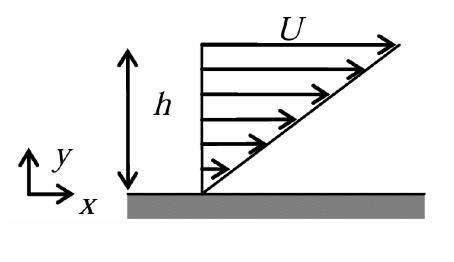
\includegraphics[width=0.35\linewidth]{./figures/f5_12.png}
\end{figure}
\bigbreak
The flow rate in the $x$ direction can be described by:
\[ 
u = U \left( \frac{y}{h} \right)
.\]
And the flow in the $y$ direction by:
\[ 
v = 0
.\]

We start by checking if the flow is incompressible:
\begin{align*}
  \frac{\partial u}{\partial x} + \frac{\partial v}{\partial y} &= 0 \\
  \frac{\partial U \left( \frac{y}{h} \right)}{\partial x} + \frac{\partial 0}{\partial y} &= 0
.\end{align*}
Hence the flow is incompressible. The stream function $\psi$ for an incompressible flow is defined by the two equations:
\[ 
u = \frac{\partial \psi}{\partial y}; \qquad v = - \frac{\partial \psi}{\partial x}
.\]
We integrate the expression for $u$ with respect to $y$ to find the stream function:
\begin{align*}
  \psi(x,y) &= \int U \frac{y}{h} \, \mathrm{d}y \\
  &= \frac{U y^2}{2 h} + f(x)
.\end{align*}
And we can also integrate the expression for $v$ with respect to $x$ to get:
\begin{align*}
  \psi(x,y) &= - \int 0 \, \mathrm{d}x  \\
            &= g(y)
.\end{align*}
As these two functions must be the same. Therefore $f(x) = 0$ and $g(y) = \frac{U 2y^2}{2h}$. The stream function therefore becomes:
\[ 
\psi(x,y) = \frac{U y^2}{2h}
.\]

The entire flow rate can be found by integrating the velocity over the entire range. In this case:
\[ 
Q = \int_{0}^{h} u \, \mathrm{d}y = \frac{U}{h} \int_{0}^{h} y \, \mathrm{d}y = \frac{U h}{2}
.\]
Now to find the $y$-value at half the flow rate we use the same formula however we plug $\frac{Q}{2}$ in at the place of the flow rate and set $h = h_{\mathrm{half}}$ as our variable as:
\begin{align*}
  \frac{Q}{2} &= \int_{0}^{h_{\mathrm{half}}} u \, \mathrm{d}y  \\
  &= \frac{U}{h} \int_{0}^{h_{\mathrm{half}}}  y \, \mathrm{d}y \\
  &= \frac{U}{h} \cdot \frac{h_{\mathrm{half}}^2}{2} \\
  \frac{Q}{2} &= \frac{1}{2} \cdot \left( \frac{U h}{2} \right) \\
  &= \frac{U \cdot h}{4} \\
  \implies \frac{U}{h} \cdot \frac{h_{\mathrm{half}}^2}{2} &= \frac{U \cdot h}{4} \\
  h_{\mathrm{half}}^2 &= \frac{h^2}{2} \\
                      &= \frac{(\qty{1,5}{m} )^2}{2} \\
                      &= \qty{1,06}{m} 
.\end{align*}

